\documentclass[12pt]{report}
\usepackage[utf8]{inputenc}
\usepackage{geometry}
\geometry{letterpaper, margin=0.25in}
\usepackage{graphicx} 
\usepackage{multicol}
\usepackage{parskip}
\usepackage{booktabs}
\usepackage{array} 
\usepackage{paralist} 
\usepackage{verbatim}
\usepackage{sectsty}
\usepackage[shortlabels]{enumitem}

\usepackage{amsmath}
\usepackage{amssymb}
\usepackage{mathtools}
\usepackage{empheq}
\usepackage{xcolor}
\usepackage{bbm}
\usepackage{tikz}
\usepackage{pgfplots}
\usepackage{tikz-cd}
\usepackage{circuitikz}
\usepackage{multirow}
\pgfplotsset{compat=1.18}
\usetikzlibrary{intersections, decorations.markings, decorations.pathmorphing}
 \usepgfplotslibrary{fillbetween}
\tikzset{
    marking along/.style n args={2}{
        decoration={
                markings, 
                mark=at position #1 with {\arrow{#2}}
        },
        postaction={decorate}
        },
    marking along/.default={0.5}{>},
    wavy/.style={
        decorate,decoration={coil,aspect=0}
     },
    two marks/.style n args={1}{
        decoration={
            markings,
            mark=at position 0.25 with {\arrow{#1}},
            mark=at position 0.75 with {\arrow{#1}}
         },
         postaction={decorate}
    },
    two marks/.default={>}
}

\colorlet{mygreen}{green!50!teal}

\newcommand{\ans}[1]{\boxed{\text{#1}}}
\newcommand{\vecs}[1]{\langle #1\rangle}
\renewcommand{\hat}[1]{\widehat{#1}}

\renewcommand{\P}{\mathbb{P}}
\newcommand{\R}{\mathbb{R}}
\newcommand{\E}{\mathbb{E}}
\newcommand{\Z}{\mathbb{Z}}
\newcommand{\N}{\mathbb{N}}
\newcommand{\Q}{\mathbb{Q}}
\newcommand{\C}{\mathbb{C}}

\newcommand{\ind}{\mathbbm{1}}
\newcommand{\qed}{\quad \blacksquare}

\newcommand{\brak}[1]{\left\langle #1 \right\rangle}
\newcommand{\bra}[1]{\left\langle #1 \right\vert}
\newcommand{\ket}[1]{\left\vert #1 \right\rangle}

\newcommand{\abs}[1]{\left\vert #1 \right\vert}
\newcommand{\mfX}{\mathfrak{X}}
\newcommand{\ep}{\varepsilon}

\newcommand{\Ec}{\mathcal{E}}
\newcommand{\Nc}{\mathcal{N}}
\newcommand{\A}{\mathcal{A}}
\newcommand{\F}{\mathcal{F}}
\newcommand{\Cc}{\mathcal{C}}
\newcommand{\B}{\mathcal{B}}
\newcommand{\M}{\mathcal{M}}
\newcommand{\X}{\chi}
\renewcommand{\L}{\mathcal{L}}

\newcommand{\sub}{\subseteq}
\newcommand{\st}{\text{ s.t. }}
\newcommand{\card}{\text{card }}
\renewcommand{\div}{\vspace*{10pt}\hrule\vspace*{10pt}}
\newcommand{\surj}{\twoheadrightarrow}
\newcommand{\inj}{\hookrightarrow}
\newcommand{\biject}{\hookrightarrow \hspace{-8pt} \rightarrow}
\renewcommand{\bar}[1]{\overline{#1}}
\newcommand{\overcirc}[1]{\overset{\circ}{#1}}
\newcommand{\diam}{\text{diam }}
\newcommand{\iid}{\overset{	ext{iid}}{\sim}}

\renewcommand{\Re}{\text{Re}\,}
\renewcommand{\Im}{\text{Im}\,}
\newcommand{\Var}{\text{Var}\,}
\newcommand{\Cov}{\text{Cov}\,}

\DeclareMathOperator*{\argmax}{\arg\max}
\DeclareMathOperator*{\argmin}{\arg\min}

\newcommand{\sign}{\text{sign}\,}

\newcommand*{\tbf}[1]{\ifmmode\mathbf{#1}\else\textbf{#1}\fi}

\usepackage{tcolorbox}
\tcbuselibrary{breakable, skins}
\tcbset{enhanced}
\newenvironment*{tbox}[2][gray]{
    \begin{tcolorbox}[
        parbox=false,
        colback=#1!5!white,
        colframe=#1!75!black,
        breakable,
        title={#2}
    ]}
    {\end{tcolorbox}}

\newenvironment*{exercise}[1][red]{
    \begin{tcolorbox}[
        parbox=false,
        colback=#1!5!white,
        colframe=#1!75!black,
        breakable
    ]}
    {\end{tcolorbox}}

\newenvironment*{proof}[1][blue]{
\begin{tcolorbox}[
    parbox=false,
    colback=#1!5!white,
    colframe=#1!75!black,
    breakable
]}
{\end{tcolorbox}}
\newenvironment*{proposition}[1][gray]{
    \begin{tcolorbox}[
        parbox=false,
        colback=#1!5!white,
        colframe=#1!75!black,
        breakable
    ]}
    {\end{tcolorbox}}


\title{ ENGN 1580 - Communications Systems}
\author{Milan Capoor}
\date{Spring 2026}

\begin{document}
\maketitle

\chapter{Fourier Transforms}
\section{Jan 22}

\subsection{Linear Systems}

What is a linear system? 
\begin{enumerate}
    \item $L[u+v] = L[u]+L[v]$ (additivity)
    \item $L[au] = aL[u]$ (scaling) 
    \item $L[ax + by] = aL[x] + bL[y]$ (superposition)
\end{enumerate}

Do we actually need scaling if we have additivity?

\emph{Example 1.} 
\[ L[x+x]= Lx + Lx = 2Lx \]
seems like  we don't. What about rationals?

\emph{Example 2.} if we want $L[0.1x]$ we can see 
\[L[x]= L[0.1x + \dots + 0.1x] = 10L[0.1x] \implies L[0.1x] = \frac{1}{10}L[x] \]
still working... 

\emph{Example 3.} And even for negatives...
\begin{gather*}
    L[-x]=L[x-x-x]=L[x]+2L[-x]
    0 = L[x]+L[-x]
    L[-x] = -L[x]
\end{gather*}

(\tbf{Remark:} this also immediately leads to the identity $L[0]=0$ for all linear systems)

\emph{Example 4 (A counter):} What if $L[ax]$ is irrational? We can approximate by rationals and apply the same arguments above but this requires $L$ continuous on $\R \setminus \Q$ -- a rather strong condition 

Where things really break are $\C$: what could we possibly say about $L[jx]$? (convention: $j$ is imaginary basis in this class)

\subsection{Periodic Signals}

\tbf{Signal:} a function 

\tbf{periodic signals:} from fourier series 
\[p(t) = \sum p_k exp(2\pi jk/T) \]
for period $T$ 
where 
\[p_k = \frac 1T \int_{-T/2}^{T/2} p(t) e^{-j * 2\pi /T * kt} \; dt\]
(as an aside notice that this is a projection) 

\tbf{Fourier transform:}
\[\mathfrak X f = \int x(t) e^{-j * 2\pi ft} \; dt \]

\tbf{Inverse Fourier:}
\[x(t) = \int \mathfrak Xf e^{j* 2\pi ft} \; df\]

where $f$ is the frequency (note we are missing the coefficients because we work in Hz) 

\tbf{Laplace:}
\[x(s) = \int x(t) e^{-st} \; dt \]

Notice that all of these transforms have integrals of exponentials. Why might that be? 

\tbf{Linear time invariant (LTI) systems:} Let L[x(t)] = y(t). If this is an LTI,
\[L[x(t-\tau)] = y(t - \tau)\]

\tbf{impulse:} square function of lengths $1/\ep$ centered at 0 satisfying 
\begin{enumerate}
    \item $\int \delta(t) \; dt = 1 $
    \item $\int \delta(t-a)s(t) \; dt = s(a) $(sifting property) 
\end{enumerate}

\begin{center}
\begin{tikzpicture}
    \draw (0, 0) -- (4, 0);
    \draw (2, 0) -- (2, 3);
    \draw[blue] (1, 0) rectangle ++(2, 2);

    \node[below] at (1, 0) {$-\ep/2$};
    \node[below] at (3, 0) {$\ep/2$};
    \node[right] at (3, 2) {$1/\ep$};
    
\end{tikzpicture}
\end{center}

This leads to an alternative definition of an LTI $h(t)$ as one for which 
\begin{enumerate}
    \item $h(\delta(t)) = h(t)$
    \item $h(a\delta(t-\tau)) =ah(t-\tau)$
\end{enumerate}

Let us consider a general case 
\[x(t) = \int x(\tau)\delta(t-\tau)d\tau\]
now what is $h(x(t))$? 

If we view the integral as a Riemann sum, we can see easily that 
\begin{align*}
    h(x(t)) &= h(\int x(\tau)\delta(t-\tau)d\tau)\\ 
    &= \int x(\tau)h(t-\tau)d\tau \\ 
    &= y(t)
\end{align*}
a convolution! (and of course we could equally see by a change of variables $\int x(t-\tau)h(\tau)d\tau$)

What about $h(e^{jst})$? 
\[\int e^{js(t-\tau)} h(\tau) d\tau= e^{jst} \int h(t) e^{-jst} d\tau\]

\section{Jan 27}

\tbf{Outline of a Communications System:}
\begin{center}
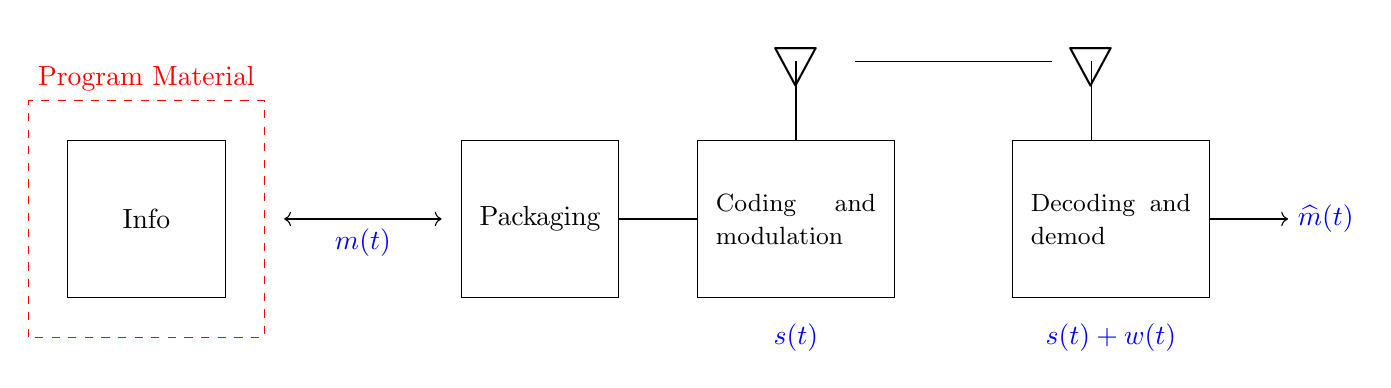
\begin{tikzpicture}

    \draw (-1, 0) rectangle ++(2, 2) node[midway] {Info};
    \draw[red, dashed] (-1.5, -0.5) rectangle ++(3, 3) node[above left] {Program Material};

    \draw[<->] (1.75, 1) -- ++(2, 0) node[midway, below, blue] {$m(t)$};
    \draw (4,0) rectangle ++(2, 2) node[midway] {Packaging};
    \draw (6, 1) -- (7, 1);
    \draw (7,0) rectangle ++(2.5, 2) node[midway] {\parbox{0.8in}{{\small Coding and modulation}}};
    \draw (8.25, 2) -- ++(0, 1) node {\rotatebox{180}{\scalebox{2}{$\triangle$}}};
    \node[blue] at (8.25, -0.5) {$s(t)$};

    \draw (9, 3) to[decorate, decoration={coil, aspect=2}] ++(2.5, 0) ;

    \draw (12, 2) -- ++(0, 1) node {\rotatebox{180}{\scalebox{2}{$\triangle$}}};
    \draw (11,0) rectangle ++(2.5, 2) node[midway] {\parbox{0.8in}{{\small Decoding and demod}}};
    \node[blue] at (12.25, -0.5) {$s(t) + w(t)$};

    \draw[->] (13.5, 1) -- ++(1, 0) node[blue, right] {$\hat m(t)$};

\end{tikzpicture}
\end{center}
where: 
\begin{itemize}
    \item info is viewed broadly as songs, video, text, etc.
    \item $m(t)$ is the message signal (assuming no loss between program material and packaging)
    \item $s(t)$ is the transmitted signal
    \item $w(t)$ is noise added by the transmission interference 
    \item $\hat m(t)$ is the received (estimated) message signal
\end{itemize}

\subsection{Linear system review:}
A system $L$ is \tbf{linear} if it satisfies \emph{superposition}: 
\[L{ax + by} = aL[x] + bL[y]\]

If we define a delta function $\delta(t)$ satisfying
\begin{enumerate}
    \item $\int_{-\infty}^{\infty} \delta(t)\; dt = \int_{0^-}^{0^+} \delta(t) \; dt = 1$
    \item $\int \delta(t-a)s(t) \; dt = s(a)$ (sifting property)
\end{enumerate}

Last time we saw the square pulse. However, we can also define it as the limit of a Gaussian as $\sigma \to 0$: 
\[\delta_{\sigma}(t) = \sqrt{\frac{1}{2\pi\sigma^2}} e^{-\frac{t^2}{2\sigma^2}}\]

\begin{center}
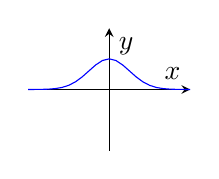
\begin{tikzpicture}
\begin{axis}[
    width=0.3\textwidth,
    axis lines=middle,
    no markers,
    xtick=\empty,
    ytick=\empty,
    clip=false,
    xlabel={$x$},
    ylabel={$y$},
    domain=-2:2,
    ymin=-2, ymax=2,
    xmin= -2, xmax=2,
    view = {0}{90}
]
    \addplot{exp(-x^2/0.5)};
\end{axis}
\end{tikzpicture}
\end{center}

\begin{exercise}
    \textbf{Exercise:} Show that $\delta_{\sigma}(t)$ is a delta function as $\sigma \to 0$. 
\end{exercise}

\tbf{Impulse response of a linear system:} 

\begin{center}
\begin{tikzpicture}
    \draw (0, 0) rectangle ++(2, 2) node[midway] {$h(t)$}; 
    \draw[<-, shorten <= 5pt] (0, 1) -- ++(-1,  0) node[left] {$\delta(t -t_0)$}; 
    \draw[->, shorten <= 5pt] (2, 1) -- ++(1, 0) node[right] {$h(t- t_0)$};
\end{tikzpicture}
\end{center}

With a little work, we can generalize this property to see that for any input signal $x(t)$, the output of a linear system is given by the convolution of the input with the impulse response:

\begin{align*}
    y(t) &= h(x(t)) \\
    &= \int_{-\infty}^{\infty} x(\tau) h(t - \tau) \; d\tau \\
    &= \int_{-\infty}^{\infty} x(t- \tau) h(\tau) \; d\tau
\end{align*}

\tbf{Fourier Transform:}
\[h(t) \overset{\F}{\implies} H(f) = \int_{-\infty}^{\infty} h(t) e^{-j\;2\pi ft}\; dt\]

\emph{Example:} Let $x(t) = \cos 2\pi f_0 t$. What is $X(f)$?
\begin{align*}
    \cos 2\pi f_0 t &= \frac{e^{j\; 2\pi f_0t} + e^{-j\; 2\pi f_0t}}{2}\\ 
    h(\cos 2\pi f_0t) &= \frac{1}{2}h(e^{j\; 2\pi f_0t}) + \frac{1}{2}h(e^{-j\; 2\pi f_0t}) \\
    &= \frac{1}{2}e^{j\; 2\pi f_0t}H(f_0) + \frac{1}{2}e^{-j\; 2\pi f_0t}H(-f_0)
\end{align*}

Let's generalize: 
\begin{align*}
    h(x(t)) &= y(t) - \int x(\tau) h(t - \tau) \; d\tau \\
    &\overset{\F}{=} \int \int x(\tau) h(t - \tau) e^{-j\; 2\pi ft} \; dt\, d\tau\\
    &= \int x(\tau) \left(\int h(t -\tau) e^{-j\; 2\pi ft}\; dt\right) \; d\tau\\ 
    &= \int x(t) \left[\int h(u) e^{-j\; 2\pi f(u + \tau)}\right]\; d\tau \qquad (u = t -\tau)\\ 
    &=  \int x(t) \underbrace{\left[\int h(u) e^{-j\; 2\pi fu}\right]}_{H(f)} e^{-j\; 2\pi f\tau}\; d\tau\\
    &\overset{\F^{-1}}= X(f)H(f)
\end{align*}

Which yields the important result: \emph{convolution in the time domain is multiplication in the frequency domain:}
\[x(t) \star h(t) = (x\star h)(t) \overset{\F}{=} X(f)H(f)\]

In fact, the work here leads to a number of useful properties of the Fourier transform:

\tbf{Time shift property:} 
\[\boxed{\F[x(t- t_0)] = e^{j\; 2\pi ft_0} X(f)}\]

\tbf{Scaling:} 
\begin{align*}
    \F[x(at)] &= \int x(at) e^{-j\; 2\pi ft}\; dt\\ 
    &= \int x(u) e^{-j\; 2\pi f(u/a)} \frac{du}{a} \qquad (du = a\; dt)\\
    &= \boxed{\frac{1}{\abs a} X(f/a) }
\end{align*}

\tbf{Differentiation:}
\begin{align*}
    \frac{d}{dt} x(t) &= \frac{d}{dt}\left[\int X(f) e^{j\; 2\pi ft}\; df\right] \\ 
    &= \int X(f)(j\; 2\pi f) e^{j\; 2\pi ft}\; dt
\end{align*}
so 
\[\boxed{\F\left[\frac{dx}{dt}\right] = X(f) \; j 2\pi f}\]

\tbf{Integration:}
\[\boxed{\F\left[\int_{-\infty}^t x(u)\; du\right] = \frac{X(f)}{j\, 2\pi f} + \frac{X(0)}{2} \delta(f)}\]

\begin{exercise}
    \textbf{Exercise:} Prove the integration property
\end{exercise}

\tbf{Parseval:}
\[\boxed{\int_{-\infty}^{\infty} x^2(t) = \Ec_x = \int_{-\infty}^{\infty} \abs{X(f)}^2 \; df}\]
(``the energy in time domain = energy in frequency domain'')

We've seen over and over that $\F[x(t)] = X(f)$? What about $\F[X(f)]$? 

First, two fact that should be obvious:
\begin{align*}
    \F[\delta(t)] &= 1\\ 
    \F[\delta(t - \tau)] &= e^{-j\; 2\pi ft}
\end{align*}
and since (up to sets of measure zero), 
\[\delta(t - \tau) \overset{\F}{\underset{\F^{-1}}{\iff}} e^{-j\; 2\pi ft}\]

which gives us 

\tbf{Duality:}
\begin{align*}
    \F[X(t)] &= \int X(t) e^{-j\; 2\pi ft}\; dt\\ 
    &= \int x(u) e^{-j\; 2\pi(-tu)} \; du\\ 
    &= \int \int x(u) e^{-j\; 2\pi tu} e^{-j\; 2\pi t}\; du\, dt\\
    &= \int x(u) \left[\int e^{-j\; 2\pi t(u+f)}\; dt\right] \; du\\ 
    &= \int x(u) \delta(u + f)\; du\\
    &= x(-f)
\end{align*}

Graphically, for a square function, 

\begin{center}
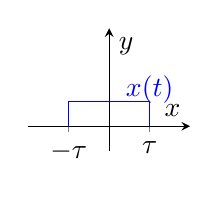
\begin{tikzpicture}
\begin{axis}[
    width=0.3\textwidth,
    axis lines=middle,
    no markers,
    xtick={-2, 2},
    xticklabels={$-\tau$, $\tau$},
    ytick={\empty},
    clip=false,
    xlabel={$x$},
    ylabel={$y$},
    domain=-2:2,
    ymin=-1, ymax=4,
    xmin= -4, xmax=4,
    view = {0}{90}
]

\addplot coordinates {(-2, 0) (-2, 1) (2, 1) (2, 0)};
\node[blue] at (2, 1.5) {$x(t)$};
\end{axis}
\end{tikzpicture}
\end{center}

\begin{align*}
    \F[x(t)] &= \int_{-T}^T e^{-j\; 2\pi ft} \;dt\\ 
    &= \left(\frac{1}{-j\, 2\pi f}\right) e^{-j\; 2\pi ft} \bigg\vert_{-T}^T\\ 
    &= -\frac{1}{j\, 2\pi f} \left(e^{-j\; 2\pi fT} - e^{j\; 2\pi fT}\right)  \\ 
    &= -\frac{1}{\pi f} \sin(-2\pi fT)  \qquad \left(\sin z = \frac{e^{jz} - e^{-jz}}{2j}\right) \\ 
    &= \frac{\sin 2\pi fT}{\pi f} \\ 
\end{align*}

\begin{center}
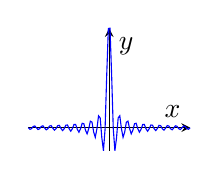
\begin{tikzpicture}
\begin{axis}[
    width=0.3\textwidth,
    axis lines=middle,
    no markers,
    xtick=\empty,
    ytick=\empty,
    clip=false,
    xlabel={$x$},
    ylabel={$y$},
    domain=-2*pi:2*pi,
    samples=100,
    view = {0}{90}
]
    \addplot {sin(10*deg(x))/(7*x)};
\end{axis}
\end{tikzpicture}
\end{center}

\section{Jan 29}

\tbf{Recall:} What is the Fourier transform of this box? 

\begin{center}
\begin{tikzpicture}
    \draw (0, 0) -- (6, 0);
    \draw (3, 0) -- (3, 3);

    \draw[blue] (1, 0) node[below] {$-T/2$} -- (1, 2) -- (5, 2) node[above right] {$1/T$} -- (5, 0) node[below] {$T/2$};
\end{tikzpicture}
\end{center}

(Note this is an impulse as $T \to 0$)

\[\F = \int_{-T/2}^{T/2} \frac{1}{T} e^{-j\; 2\pi ft}\; dt = \frac{1}{T} \left(\frac{1}{-j\, 2\pi f}\right) e^{-j\; 2\pi ft} \bigg\vert_{-T/2}^{T/2} = \frac{1}{-j\, 2\pi f T} \left(e^{-j\; \pi f T} - e^{j\; \pi f T}\right) = \frac{\sin(\pi f T)}{\pi f T} \]

How might we sanity check this? 

We already saw that as $T \to 0$, this becomes an impulse in the time domain. What happens in the frequency domain?
\[\lim_{T \to 0} \frac{\sin \pi f T}{\pi f T} = 1\]
and indeed this matches the rule $\F(\delta(t)) = 1$.

\emph{Example:} 
\[\F[e^{-at}u(t)] = \int_0^{\infty} e^{-at} e^{-j\; 2\pi ft}\; dt
    = \int_0^{\infty} e^{-(a + j\; 2\pi f)t}\; dt
    = \frac{1}{a + j\; 2\pi f}
\]
(for $a > 0$ and $u(t)$ the unit step function)

\tbf{Convolution:} 
\[\int_{-\infty}^{\infty} x(\tau) y(t -\tau)\; d\tau\]

\emph{Example:} Convolve two box functions of width $2$:

\begin{center}
\begin{tikzpicture}[scale=0.7]
    \draw (0, 0) -- (6, 0);
    \draw (3, 0) -- (3, 3);

    \draw[blue] (1, 0) node[below] {$-1$} -- (1, 2) -- (5, 2) node[above right] {$x(t)$} -- (5, 0) node[below] {$1$};

    \node at (7, 1) {\scalebox{2.5}{$\star$}};

    \draw (8, 0) -- (14, 0);
    \draw (11, 0) -- (11, 3);

    \draw[red] (9, 0) node[below] {$-1$} -- (9, 2) -- (13, 2) node[above right] {$y(t)$} -- (13, 0) node[below] {$1$};
\end{tikzpicture}
\end{center}

We could do this directly or we can think about it geometrically.

$y(t - \tau)$ corresponds to a reflection and shift by $t$. 

\begin{center}
\begin{tikzpicture}[scale=0.7]
    \draw (-6, 0) -- (6, 0);
    \draw (3, 0) -- (3, 3);

    \draw[blue] (1, 0) node[below] {$-1$} -- (1, 2) -- (5, 2) node[above right] {$x(t)$} -- (5, 0) node[below] {$1$};

    \draw[red] (-5, 0) node[below] {$t-1$} -- (-5, 2) -- (-1, 2) node[above] {$y(t)$} -- (-1, 0) node[below] {$t+1$};
\end{tikzpicture}
\end{center}

Clearly, multiplying these two functions will give nonzero output only when they overlap. When do they overlap? Precisely at $t \in (-2, 2)$.

\begin{center}
\begin{tikzpicture}
     \draw (-3, 0) -- (3, 0);
    \draw (0, 0) -- (0, 3);

    \draw (-2, 0) node[below] {$-2$} -- (0, 2) node[above right] {$2$} -- (2, 0) node[below] {$-2$};
\end{tikzpicture}
\end{center}

Notice that the length of the domain was 2 before convolving and 4 after convolving. This makes sense since convolution is a ``spreading and smoothing'' operation 

\emph{Example:} $\delta(t) \star x(t)$ where $x(t)$ 

\begin{center}
\begin{tikzpicture}
    \draw (-3, 0) -- (3, 0);
    \draw (0, -2) -- (0, 2);

    \draw[blue] plot[smooth, tension=2] coordinates {(-2, 0) (-1.5, -0.25) (-1, 1) (0, 0) (1, -1) (2, 0)} node[above right] {$x(t)$};
\end{tikzpicture}
\end{center}

Trick question! 
\[\int \delta(x - \tau) x(\tau) \; d\tau = x(t)\]
(sifting!) 

For this class, we should think about convolutions critically and graphically: 

\begin{center}
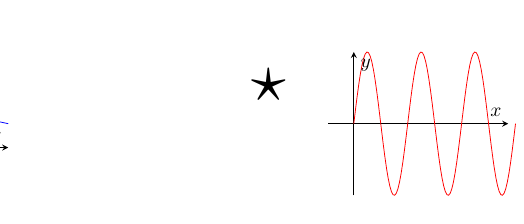
\begin{tikzpicture}[scale=0.7]
    \hspace{-1in}\begin{axis}[
        width=0.4\textwidth,
        axis lines=middle,
        no markers,
        xtick=\empty,
        ytick=\empty,
        clip=false,
        xlabel={$x$},
        ylabel={$y$},
        domain=-2:2,
        ymin=-1, ymax=2,
        xmin= -1, xmax=2,
        view = {0}{90}
    ]

    \addplot[domain=0.4:2, blue] {1/x};
    \end{axis}

    \node at (8, 2) {\scalebox{2.5}{$\star$}};

    \hspace{2.5in}\begin{axis}[
        width=0.4\textwidth,
        axis lines=middle,
        no markers,
        xtick=\empty,
        ytick=\empty,
        clip=false,
        xlabel={$x$},
        ylabel={$y$},
        xmin=-1, xmax=6,
        ymin=-1, ymax=1,
        view = {0}{90}
    ]

    \addplot[domain=0:2*pi, samples=100, red] {sin(3*deg(x))};
    \end{axis}
\end{tikzpicture}
\end{center}

What is the convolution of these two functions at $t= -2$? 

These would be quite annoying to do directly but if we notice that $\textcolor{blue}{x(t)}$ is undefined for $t \leq 0$ then we can see that there is no overlap at all and the convolution is 0.

\begin{proposition}
    \textbf{Recall:} 
    \begin{align*}
        \F(x(t)) &= X(f)\\ 
        \F(X(t)) &= x(-f)\\ 
        \F(\delta(t)) &= 1
    \end{align*}
    so 
    \begin{align*}
        \F(\delta(t- t_0)) &= e^{-j\; 2\pi ft_0}\\ 
        \F(e^{-j\; 2\pi f_0t}) &= \delta(f+ f_0)
    \end{align*}
\end{proposition}

\emph{Example:} $\F(\cos 2\pi f_0 t)$ does not converge analytically BUT 

\[\cos 2\pi f_0 t = \frac{e^{j\; 2\pi f_0t} + e^{-j\; 2\pi f_0t}}{2}\]
so from the above, 

\begin{center}
\begin{tikzpicture}
    \draw (-3, 0) -- (3, 0);
    \draw (0, -1) -- (0, 2);
    \draw (-0.1, 1) -- (0.1, 1) node[above right] {$1/2$};

    \draw[blue, <-] (-2, 1) -- (-2, 0) node[below] {$-f_0$};
    \draw[blue, <-] (2, 1) -- (2, 0) node[below] {$f_0$};
\end{tikzpicture}
\end{center}

Similarly, 
\begin{align*}
    \F(\sin 2\pi f_0 t) &= \F\left(\frac{1}{2j} e^{j\; 2\pi f_0t} - e^{-j\; 2\pi f_0t}\right)\\ 
    &= \frac{1}{2j}(\delta(f + f_0) - \delta(f - f_0))
\end{align*}

\begin{center}
\begin{tikzpicture}
    \draw (-3, 0) -- (3, 0);
    \draw (0, -1) -- (0, 2);
    \draw (-0.1, 1) -- (0.1, 1) node[above right] {$1/2j$};

    \draw[blue, <-] (-2, -1) -- (-2, 0) node[above] {$-f_0$};
    \draw[blue, <-] (2, 1) -- (2, 0) node[below] {$f_0$};
\end{tikzpicture}
\end{center}

\tbf{Complex conjugation:} $(a + bj)^* = a - bj$

We know 
\[\F(x(t)) = \int x(t) e^{-j\; 2\pi ft}\; dt = X(f)\]
so what is $\F(x^*(t))$?
\begin{align*}
    F(x^*(t)) &= \int x^*(t) e^{j\; 2\pi ft}\; dt\\
    &= \int x^*(t) e^{-j\; 2\pi (-f)t}\; dt\\
    &= X(-f)\\ 
    &= X^*(f)
\end{align*}

leading to the property:
\[\boxed{X^*(f) = X(-f)}\]

\tbf{Even/Odd Property:} Let $x(t) = x(-t)$. Then 
\[\int_{-\infty}^{\infty} x(t) e^{-j\; 2\pi ft}\; dt = \int_0^{\infty} x(t) e^{-j\; 2\pi ft} + x(t) e^{j\; 2\pi ft}\; dt = 2\int_0^{\infty} x(t) \cos 2\pi ft\; dt \in \R\]

\emph{Even functions have real fourier transforms. Odd functions have imaginary fourier transforms.}

\section{Linear Systems Assessment}

\begin{exercise}
    \textbf{Exercise:} The Fourier transform of $x(t)$ is $X(f)$. Prove that the Fourier transform of $x(t - t_0)$ is $e^{-j\; 2\pi ft_0} X(f)$. 
\end{exercise}

\begin{exercise}
    \textbf{Exercise:} The energy in a signal $x(t)$ is defined as 
    \[E = \int_{-\infty}^{\infty} \abs{x(t)}^2\; dt\]
    Prove that if $X(f)$ is the Fourier transform of $x(t)$, then we must also have 
    \[E = \int_{-\infty}^{\infty} \abs{X(f)}^2 \; df\]

    \emph{Hint:} You may use the fact that 
    \[\int_{-\infty}^{\infty} e^{j\; 2\pi vt}\; dt = \delta(v)\]
\end{exercise}

\begin{exercise}
    \textbf{Exercise:} A signal $x(t)$ of finite energy is applied to a square-law device whose output is defined by $y(t) = x^2(t)$. The spectrum $X(f)$ of $x(t)$ is limited to the frequency interval $-W \leq f \leq W$. Show that the spectrum, $Y(f)$ of $y(t)$ is limited to the frequency interval $-2W \leq f \leq 2W$.
\end{exercise}

\begin{exercise}
    \textbf{Exercise:} Show that the overall transfer function $H(s)$ for the feedback system below is given by 
    \[H(s) = \frac{F(s)}{1 - F(s) G(s)}\]

    \begin{center}
        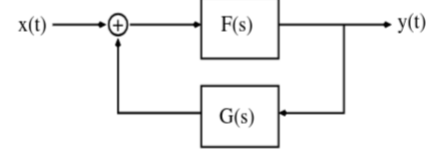
\includegraphics[width=0.5\textwidth]{Images/feedback_system.png}
    \end{center}
\end{exercise}
\chapter{Modulation}

Consider a simple modulation and demodulation scheme:
\begin{center}
\begin{tikzpicture}

    \node[blue] at (0.5, 0) {$m(t)$};

    \begin{axis}[
        at={(-1cm,-2.5cm)},
        width=0.2\textwidth,
        axis lines=middle,
        no markers,
        xtick=\empty,
        ytick=\empty,
        clip=false,
        xlabel={},
        ylabel={},
        domain=0.2:1.8,
        ymin=-1, ymax=3,
        xmin= -1, xmax=2,
        view = {0}{90}
    ]
        \addplot[blue] {(x-1)^2+1};
    \end{axis}

    \draw[->] (1, 0) -- ++(1, 0); 
    \draw (2.5, 0) circle (10pt) node {$\times$};
    \draw[<-] (2.5, -0.5) -- ++(0, -1.5) node[below] {$\cos 2\pi f_c t$};
    \draw (2.5, 0.5) -- ++(0, 1) node {\rotatebox{180}{\scalebox{2}{$\triangle$}}};
    \draw[dashed] (3, 1.5) -- ++(0.5, 0) node[right, blue] {$m(t) \cos 2\pi f_c t$};

    \begin{axis}[
        at={(3.5cm,-1cm)},
        width=0.2\textwidth,
        axis lines=middle,
        no markers,
        xtick=\empty,
        ytick=\empty,
        clip=false,
        xlabel={},
        ylabel={},
        domain=0.2:1.8,
        ymin=-3, ymax=3,
        xmin= -1, xmax=2,
        view = {0}{90}
    ]
        \addplot[blue, name path=p1] {(x-1)^2+1};
        \addplot[blue, name path=p2] {-(x-1)^2-1};
        \addplot[fill=blue, fill opacity=0.1] fill between[of=p1 and p2];

    \end{axis}

    \draw[dashed] (6.5, 1.5) -- ++(0.5, 0);
    \draw (7.5, 1.5) node {\rotatebox{180}{\scalebox{2}{$\triangle$}}} -- ++(0, -1);
    \draw (7.5, 0) circle (10pt) node {$\times$};
    \draw[<-] (7.5, -0.5) -- ++(0, -1.5) node[below] {$\cos 2\pi f_c t$};
    \draw[->] (8, 0) -- ++(0.5, 0) node[right, blue] {\scalebox{1.3}{$\begin{subarray}{l}
        m(t)\cos^2 2\pi f_c t\\ 
        =\frac{m(t)}{2} + \frac{m(t)\cos 2\pi f_c t}{2}
    \end{subarray}$}};

    \draw[->] (12.5, 0) -- ++(0.5, 0);
    \draw (13.5, -1.3) rectangle ++(2, 2.5) node[midway, yshift=0.7cm] {LPF};
    \draw[->] (16, 0) -- ++(0.5, 0) node[right, blue] {$\frac{m(t)}{2}$};

    \begin{axis}[
        at={(13.75cm,-1cm)},
        width=0.15\textwidth,
        axis lines=middle,
        no markers,
        xtick=\empty,
        ytick=\empty,
        clip=false,
        xlabel={},
        ylabel={},
        domain=0.2:1.8,
        ymin=-1, ymax=2,
        xmin= -2, xmax=2,
        view = {0}{90}
    ]
        \addplot[blue] coordinates {(-1, 0) (-1, 1) (1, 1) (1, 0)};
    \end{axis}
\end{tikzpicture}
\end{center}

for $m(t)$ a message and $f_c$ a carrier frequency ($f_c \gg B$, the bandwidth of $m(t)$) which transmits the message better since it is higher frequency.

What exactly is happening here? Let's look in the frequency domain:

\begin{enumerate}
    \item Modulation:
        
    \begin{center}
    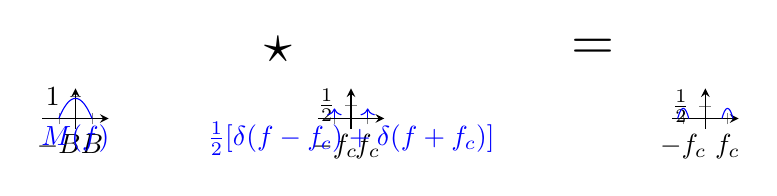
\begin{tikzpicture}
        \begin{axis}[
            at={(0cm,0cm)},
            width=0.2\textwidth,
            axis lines=middle,
            no markers,
            xtick={-1, 1},
            xticklabels={$-B$, $B$},
            ytick={2.2},
            yticklabels={1},
            clip=false,
            xlabel={},
            ylabel={},
            domain=-1:1,
            ymin=-1, ymax=3,
            xmin= -2, xmax=2,
            view = {0}{90}
        ]
            \addplot[blue] {-2*x^2+2};
            \node at (axis cs:0,-2) [blue] {$M(f)$};
        \end{axis}

        \node at (3, 1) {\scalebox{2}{$\star$}};

        \begin{axis}[
            at={(3.5cm,0cm)},
            width=0.2\textwidth,
            axis lines=middle,
            no markers,
            xtick={-1, 1},
            xticklabels={$-f_c$, $f_c$},
            ytick={1.3},
            yticklabels={$\frac{1}{2}$},
            clip=false,
            xlabel={},
            ylabel={},
            domain=-1:1,
            ymin=-1, ymax=3,
            xmin= -2, xmax=2,
            view = {0}{90}
        ]
        \draw[blue, ->] (-1, 0) -- (-1, 1);  
        \draw[blue, ->] (1, 0) -- (1, 1);  

        \node at (axis cs:0,-2) [blue] {$\frac{1}{2}[\delta(f-f_c) + \delta(f+f_c)]$};
        \end{axis}

        \node at (7, 1) {\scalebox{2}{$=$}};

        \begin{axis}[
            at={(8cm,0cm)},
            width=0.2\textwidth,
            axis lines=middle,
            no markers,
            xtick={-4, 4},
            xticklabels={$-f_c$, $f_c$},
            ytick={1.2},
            yticklabels={$\frac{1}{2}$},
            clip=false,
            xlabel={},
            ylabel={},
            ymin=-1, ymax=3,
            xmin= -6, xmax=6,
            view = {0}{90}
        ]
            \addplot[domain=-5:-3, blue] {-(x+4)^2+1};
            \addplot[domain=3:5, blue] {-(x-4)^2+1};

        \end{axis}    
    \end{tikzpicture}
    \end{center}

    Convolving with an impulse shifts the signal to be centered at the impulse!

    \item Demodulation:
    \begin{center}
    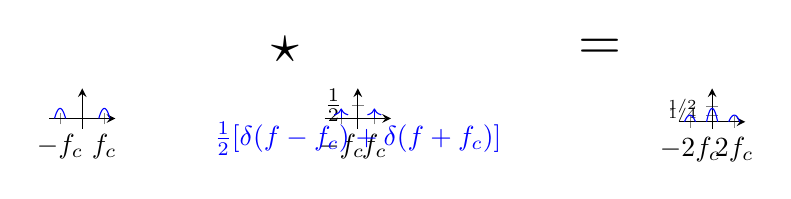
\begin{tikzpicture}
        \begin{axis}[
            at={(0cm,0cm)},
            width=0.2\textwidth,
            axis lines=middle,
            no markers,
            xtick={-4, 4},
            xticklabels={$-f_c$, $f_c$},
            ytick=\empty,
            clip=false,
            xlabel={},
            ylabel={},
            ymin=-1, ymax=3,
            xmin= -6, xmax=6,
            view = {0}{90}
        ]
            \addplot[domain=-5:-3, blue] {-(x+4)^2+1};
            \addplot[domain=3:5, blue] {-(x-4)^2+1};

        \end{axis}    

        \node at (3, 1) {\scalebox{2}{$\star$}};

        \begin{axis}[
            at={(3.5cm,0cm)},
            width=0.2\textwidth,
            axis lines=middle,
            no markers,
            xtick={-1, 1},
            xticklabels={$-f_c$, $f_c$},
            ytick={1.3},
            yticklabels={$\frac{1}{2}$},
            clip=false,
            xlabel={},
            ylabel={},
            domain=-1:1,
            ymin=-1, ymax=3,
            xmin= -2, xmax=2,
            view = {0}{90}
        ]
        \draw[blue, ->] (-1, 0) -- (-1, 1);  
        \draw[blue, ->] (1, 0) -- (1, 1);  

        \node at (axis cs:0,-2) [blue] {$\frac{1}{2}[\delta(f-f_c) + \delta(f+f_c)]$};
        \end{axis}

        \node at (7, 1) {\scalebox{2}{$=$}};

        \begin{axis}[
            at={(8cm,0cm)},
            width=0.2\textwidth,
            axis lines=middle,
            no markers,
            xtick={-4, 4},
            xticklabels={$-2f_c$, $2f_c$},
            ytick={1, 2.3},
            yticklabels={{\tiny 1/4}, {\tiny 1/2}},
            clip=false,
            xlabel={},
            ylabel={},
            ymin=-1, ymax=5,
            xmin= -6, xmax=6,
            view = {0}{90}
        ]
            \addplot[domain=-5:-3, blue] {-(x+4)^2+1};
            \addplot[domain=3:5, blue] {-(x-4)^2+1};
            \addplot[domain=-1:1, blue] {-2*x^2+2};
        \end{axis}    
    \end{tikzpicture}
    \end{center}

    (spread a copy of the signal around $-f_c$ and $f_c$ so that the interference terms reinforce each other at the baseband)

    \item Filtering:

    \begin{center}
    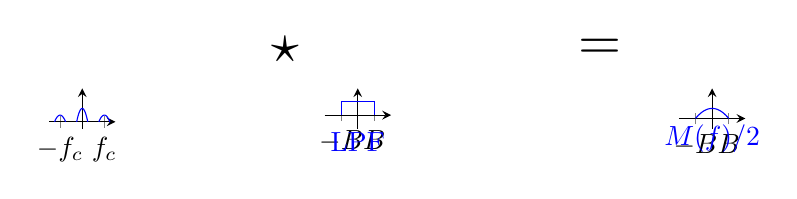
\begin{tikzpicture}
        \begin{axis}[
            at={(0cm,0cm)},
            width=0.2\textwidth,
            axis lines=middle,
            no markers,
            xtick={-4, 4},
            xticklabels={$-f_c$, $f_c$},
            ytick=\empty,
            clip=false,
            xlabel={},
            ylabel={},
            ymin=-1, ymax=5,
            xmin= -6, xmax=6,
            view = {0}{90}
        ]
            \addplot[domain=-5:-3, blue] {-(x+4)^2+1};
            \addplot[domain=3:5, blue] {-(x-4)^2+1};
            \addplot[domain=-1:1, blue] {-2*x^2+2};
        \end{axis}  

        \node at (3, 1) {\scalebox{2}{$\star$}};

        \begin{axis}[
            at={(3.5cm,0cm)},
            width=0.2\textwidth,
            axis lines=middle,
            no markers,
            xtick={-2, 2},
            xticklabels={$-B$, $B$},
            ytick=\empty,
            clip=false,
            xlabel={},
            ylabel={},
            ymin=-1, ymax=2,
            xmin= -4, xmax=4,
            view = {0}{90}
        ]
            \addplot[blue] coordinates {(-2, 0) (-2, 1) (2, 1) (2, 0)};
            \node at (axis cs:0,-2) [blue] {LPF};
        \end{axis}

        \node at (7, 1) {\scalebox{2}{$=$}};

        \begin{axis}[
            at={(8cm,0cm)},
            width=0.2\textwidth,
            axis lines=middle,
            no markers,
            xtick={-1, 1},
            xticklabels={$-B$, $B$},
            ytick=\empty,
            clip=false,
            xlabel={},
            ylabel={},
            domain=-1:1,
            ymin=-1, ymax=3,
            xmin= -2, xmax=2,
            view = {0}{90}
        ]
            \addplot[blue] {-x^2+1};
            \node at (axis cs:0,-2) [blue] {$M(f)/2$};
        \end{axis}

    \end{tikzpicture}
    \end{center}
\end{enumerate}

\section{Feb 3}

\tbf{Coherent AM:} Synchronous modulation; Modulate with $\cos 2\pi f_c t$ and demodulate with the same signal.

Recall in our demodulation step we multiplied by $\cos 2\pi f_c t$ again. What if we made a mistake and used $\sin(2\pi f_c t)$ instead? 

    \begin{center}
    \begin{tikzpicture}
        \begin{axis}[
            at={(0cm,0cm)},
            width=0.2\textwidth,
            axis lines=middle,
            no markers,
            xtick={-4, 4},
            xticklabels={$-f_c$, $f_c$},
            ytick=\empty,
            clip=false,
            xlabel={},
            ylabel={},
            ymin=-1, ymax=3,
            xmin= -6, xmax=6,
            view = {0}{90}
        ]
            \addplot[domain=-5:-3, blue] {-(x+4)^2+1};
            \addplot[domain=3:5, blue] {-(x-4)^2+1};

        \end{axis}    

        \node at (3, 1) {\scalebox{2}{$\star$}};

        \begin{axis}[
            at={(3.5cm,0cm)},
            width=0.2\textwidth,
            axis lines=middle,
            no markers,
            xtick={-1, 1},
            xticklabels={$-f_c$, $f_c$},
            ytick={1.3},
            yticklabels={$\frac{1}{2}$},
            clip=false,
            xlabel={},
            ylabel={},
            domain=-1:1,
            ymin=-2, ymax=3,
            xmin= -2, xmax=2,
            view = {0}{90}
        ]
        \draw[blue, ->] (-1, 0) -- (-1, -1);  
        \draw[blue, ->] (1, 0) -- (1, 1);  

        \node at (axis cs:0,-4) [blue] {$\begin{subarray}{c}
            \F(\sin 2\pi f_c t) = \\ 
            \frac{1}{2j}[\delta(f-f_c) - \delta(f+f_c)]
            
        \end{subarray}$};
        \end{axis}

        \node at (7, 1) {\scalebox{2}{$=$}};

        \begin{axis}[
            at={(8cm,0cm)},
            width=0.2\textwidth,
            axis lines=middle,
            no markers,
            xtick={-4, 4},
            ytick=\empty,
            xticklabels={$-2f_c$, $2f_c$},
            clip=false,
            xlabel={},
            ylabel={},
            ymin=-3, ymax=5,
            xmin= -6, xmax=6,
            view = {0}{90}
        ]
            \addplot[domain=-5:-3, red] {(x+4)^2-1};
            \addplot[domain=-1:1, red] {x^2-1};

            \addplot[domain=3:5, blue] {-(x-4)^2+1};
            \addplot[domain=-1:1, blue] {-x^2+1};
        \end{axis}    
    \end{tikzpicture}
    \end{center}

    So the signals cancel around the baseband and we get no message after filtering!

    How could we recover if we made this mistake? 

    Let's try broadcasting two messages $m_1(t) \cos 2\pi f_c t$ and $m_2(t) \sin 2\pi f_c t$ simultaneously.

    The received signal is $(s_1(t) + s_2(t))$. If we demodulate by $\cos 2\pi f_c t$ on one rail and $\sin 2\pi f_c t$ on the other rail and filter, we get two separate messages back, $m_1(t)/2$ and $m_2(t)/2$ respectively! 

    \begin{center}
    \begin{tikzpicture}
       
    \node at (0.5, 0) [blue] {$m_1(t)$};
    \draw[->] (1, 0) -- ++(1, 0); 
    \draw (2.5, 0) circle (10pt) node {$\times$};
    \draw[<-] (2.5, -0.5) -- ++(0, -0.5) node[below] {$\cos 2\pi f_c t$};
    \draw (2.5, 0.5) -- ++(0, 1) node {\rotatebox{180}{\scalebox{2}{$\triangle$}}};
    \draw[dashed] (3, 1.5) -- ++(0.5, 0) node[right, blue] {$s_1(t)$};

    \node at (0.5, -4) [blue] {$m_2(t)$};
    \draw[->] (1, -4) -- ++(1, 0); 
    \draw (2.5, -4) circle (10pt) node {$\times$};
    \draw[<-] (2.5, -4.5) -- ++(0, -0.5) node[below] {$\sin 2\pi f_c t$};
    \draw (2.5, -3.5) -- ++(0, 1) node {\rotatebox{180}{\scalebox{2}{$\triangle$}}};
    \draw[dashed] (3, -2.5) -- ++(0.5, 0) node[right, blue] {$s_2(t)$};

    \draw[dashed] (7.5, 0)  node[left, blue] {$s_1(t) + s_2(t)$} -- ++(0.5, 0);
    \draw (8.5, 0) node {\rotatebox{180}{\scalebox{2}{$\triangle$}}} -- ++(0, -4);

    \draw[->] (8.5, -1) -- ++(1, 0); 
    \draw (10, -1) circle (10pt) node {$\times$};
    \draw[<-] (10, -1.5) -- ++(0, -0.5) node[below] {$\cos 2\pi f_c t$};
    \draw (10.5, -1) -- ++(1, 0) node[right, draw, rectangle] {LPF};
    \draw (12.75, -1) -- ++(1, 0) node[right, blue] {$\frac{m_1(t)}{2}$};

    \draw[->] (8.5, -4) -- ++(1, 0); 
    \draw (10, -4) circle (10pt) node {$\times$};
    \draw[<-] (10, -4.5) -- ++(0, -0.5) node[below] {$\sin 2\pi f_c t$};
    \draw (10.5, -4) -- ++(1, 0) node[right, draw, rectangle] {LPF};
    \draw (12.75, -4) -- ++(1, 0) node[right, blue] {$\frac{m_2(t)}{2}$};

    \end{tikzpicture}
    \end{center}

    \tbf{Single sideband modulation:} Let $m(t)$ be a real signal with Fourier transform $M(f)$. We know 
    \begin{align*}
        M(f) &= \int m(t) e^{-j\; 2\pi ft}\; dt\\ 
        M^*(f) &= \int m(t) e^{-j\; 2\pi (-f)t}\; dt = M(-f)
    \end{align*}
    (i.e. the real part is even and the imaginary part is odd)

    In particular, this means we can send less information by sending only the positive frequencies or only the negative frequencies and reconstructing the other half using the even/odd properties.

    Consider:
    \begin{center}
    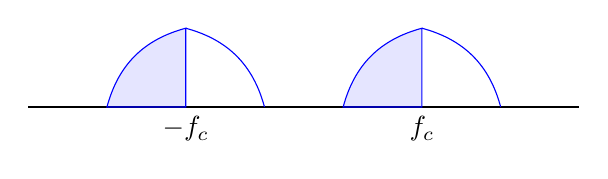
\begin{tikzpicture}
        \draw (0, 0) -- (7, 0);

        \draw[fill, blue, fill opacity=0.1] (1, 0) to[bend left] ++(1, 1) -- ++(0, -1) -- ++(-1, 0) -- cycle;
        \draw[blue]  (2, 1) to[bend left] ++(1, -1);
        \node[below] at (2, 0) {$-f_c$};


        \draw[fill, blue, fill opacity=0.1] (4, 0) to[bend left] ++(1, 1) -- ++(0, -1) -- ++(-1, 0) -- cycle;
        \draw[blue]  (5, 1) to[bend left] ++(1, -1);
        \node[below] at (5, 0) {$f_c$};


    \end{tikzpicture}
    \end{center}

    We filter, 

      \begin{center}
    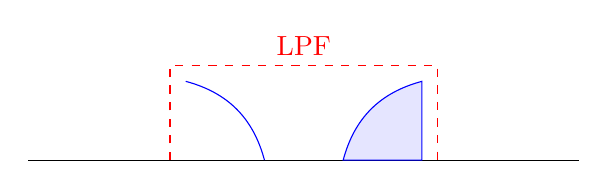
\begin{tikzpicture}
        \draw (0, 0) -- (7, 0);

        \draw[blue]  (2, 1) to[bend left] ++(1, -1);
        \draw[fill, blue, fill opacity=0.1] (4, 0) to[bend left] ++(1, 1) -- ++(0, -1) -- ++(-1, 0) -- cycle;

        \draw[dashed, red] (1.8, 0) -- ++(0, 1.2) -- node[midway, above] {LPF} ++(3.4, 0) -- ++(0, -1.2);
    \end{tikzpicture}
    \end{center}

    Then modulate by $\cos 2\pi f_c t$: 
    
    \begin{center}
    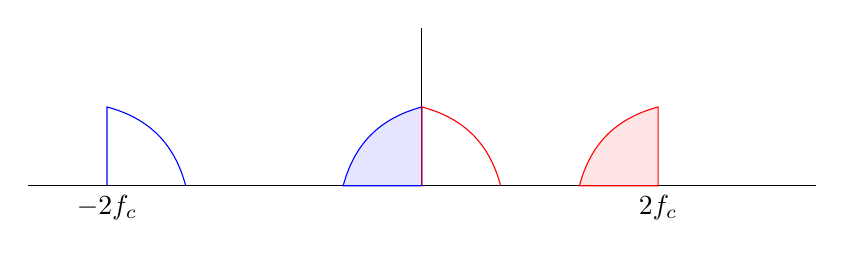
\begin{tikzpicture}
        \draw (0, 0) -- (10, 0);
        \draw (5, 0) -- ++(0, 2);

        \draw[blue] (1, 0) -- (1, 1) to[bend left] ++(1, -1); 
        
        \draw[fill, blue, fill opacity=0.1] (4, 0) to[bend left] ++(1, 1) -- ++(0, -1) -- ++(-1, 0) -- cycle;
        \draw[red] (5, 0) -- ++(0, 1) to[bend left] ++(1, -1); 
        \draw[fill, red, fill opacity=0.1] (7, 0) to[bend left] ++(1, 1) -- ++(0, -1) -- ++(-1, 0) -- cycle;

        \node[below] at (1, 0) {$-2f_c$};
        \node[below] at (8, 0) {$2f_c$};
    \end{tikzpicture}
    \end{center}

    and just like that, we have recovered the full signal using half the bandwidth!

    In practice, we can use two signals (an upper and lower sideband): 

    \begin{center}
    \begin{tikzpicture}
        \node at (0, 0) [red] {$m_1(t)$};
        \draw[->, shorten >= 5pt, shorten <= 5pt] (0.5, 0) --  ++(1, 0) node[right, draw, rectangle] {\begin{tabular}{c}
            U\\ 
            SSB 
        \end{tabular}};
        \draw (2.3, 0.8) -- ++(0, 1) node {\scalebox{2}{\rotatebox{180}{$\triangle$}}}; 

        \node at (0, -4) [blue] {$m_2(t)$};
        \draw[->, shorten >= 5pt, shorten <= 5pt] (0.5, -4) --  ++(1, 0) node[right, draw, rectangle] {\begin{tabular}{c}
            L\\ 
            SSB 
        \end{tabular}};
        \draw (2.3, -3.2) -- ++(0, 1) node {\scalebox{2}{\rotatebox{180}{$\triangle$}}}; 

        \draw (-1, 1) -- ++(2, 0);
        \draw (0, 1) -- ++(0, 1);
        \draw[red, decoration=coil, decorate] (-0.7, 1.5) -- ++(1.4, 0);
        \draw[red] (-0.7, 1) -- ++(0, 0.5);
        \draw[red] (0.7, 1) -- ++(0, 0.5);

        \draw (-1, -3) -- ++(2, 0);
        \draw (0, -3) -- ++(0, 1);
        \draw[blue] (-0.5, -3) arc (180:0:0.5 and 0.8);

        \draw (4, 0) -- ++(3, 0);
        \draw (5.5, 0) -- ++(0, 1);
        \draw[red, decoration=coil, decorate] (4.1, 0.5) -- (4.8, 0.5);
        \draw[red] (4.1, 0.5) -- ++(0, -0.5);
        \draw[red] (4.8, 0.5) -- ++(0, -0.5) node[below, black] {$-f_c$} ;
        
        \draw[red, decoration=coil, decorate] (6.2, 0.5) -- (6.9, 0.5);
        \draw[red] (6.2, 0.5) -- ++(0, -0.5) node[below, black] {$f_c$};
        \draw[red] (6.9, 0.5) -- ++(0, -0.5) ;    
        \draw[red] (-0.7, 1) -- ++(0, 0.5);
        \draw[red] (0.7, 1) -- ++(0, 0.5);

        \draw (4, -4) -- ++(3, 0);
        \draw (5.5, -4) -- ++(0, 1);
        \draw[blue] (4.8, -4) node[black, below] {$-f_c$} -- ++(0, 0.5) to[bend left] ++(0.5, -0.5);
        \draw[blue] (6.2, -4) node[black, below] {$-f_c$} -- ++(0, 0.5) to[bend right] ++(-0.5, -0.5);
    \end{tikzpicture}
    \end{center}

    

    \tbf{Frequency Division Multiplexing:}

    Define two signals $m_1(t)$ and $m_2(t)$. 

    \begin{center}
        \begin{multicols}{2}
            \begin{tikzpicture}
            \draw (0, 0) -- (4, 0) node[right] {$f$};
            \draw (2, 2) -- ++(0, -2) node[below] {$M_1(f)$};
            \draw[blue] (1, 0) to[bend left] ++(1, 1) to[bend left] ++(1, -1);
        \end{tikzpicture}

        \begin{tikzpicture}
            \draw (0, 0) -- (4, 0) node[right] {$f$};
            \draw (2, 2) -- ++(0, -2) node[below] {$M_2(f)$};
            \draw[blue] (1, 0) -- ++(1, 1) -- ++(1, -1);
        \end{tikzpicture}
        \end{multicols}
    \end{center}


    \begin{center}
    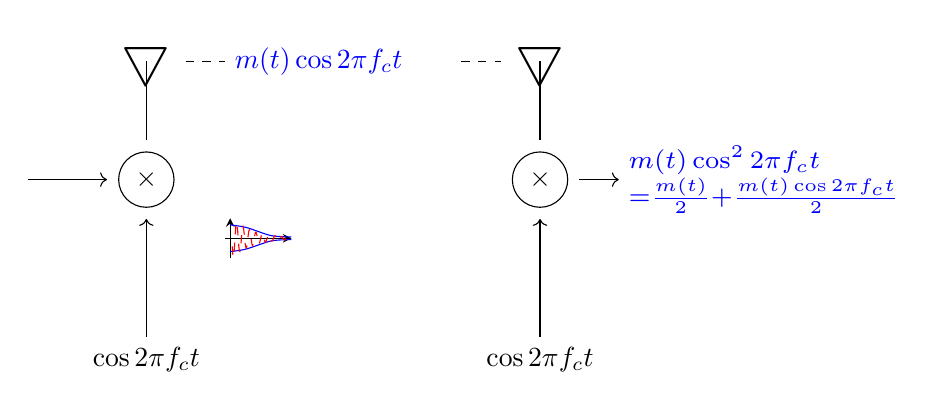
\begin{tikzpicture}
        \draw[->] (1, 0) -- ++(1, 0); 
        \draw (2.5, 0) circle (10pt) node {$\times$};
        \draw[<-] (2.5, -0.5) -- ++(0, -1.5) node[below] {$\cos 2\pi f_c t$};
        \draw (2.5, 0.5) -- ++(0, 1) node {\rotatebox{180}{\scalebox{2}{$\triangle$}}};
        \draw[dashed] (3, 1.5) -- ++(0.5, 0) node[right, blue] {$m(t) \cos 2\pi f_c t$};

        \draw[dashed] (6.5, 1.5) -- ++(0.5, 0);
        \draw (7.5, 1.5) node {\rotatebox{180}{\scalebox{2}{$\triangle$}}} -- ++(0, -1);
        \draw (7.5, 0) circle (10pt) node {$\times$};
        \draw[<-] (7.5, -0.5) -- ++(0, -1.5) node[below] {$\cos 2\pi f_c t$};
        \draw[->] (8, 0) -- ++(0.5, 0) node[right, blue] {\scalebox{1.3}{$\begin{subarray}{l}
            m(t)\cos^2 2\pi f_c t\\ 
            =\frac{m(t)}{2} + \frac{m(t)\cos 2\pi f_c t}{2}
        \end{subarray}$}};

  
        \begin{axis}[
            width=0.2\textwidth,
            at={(3.5cm,-1cm)},
            axis lines=middle,
            no markers,
            xtick=\empty,
            ytick=\empty,
            clip=false,
            xlabel={},
            ylabel={},
            domain=-2:2,
            ymin=-1.5, ymax=1.5,
            xmin= -0.25, xmax=3,
            view = {0}{90}
        ]

        \addplot[smooth, blue] coordinates {(0, 1) (0.8, 0.8) (2, 0.2) (3, 0.1)};
        \addplot[smooth, blue] coordinates {(0, -1) (0.8, -0.8) (2, -0.2) (3, -0.1)};

        \addplot[red, dashed, domain=0.1:3, samples=100] {0.6*exp(1-x) * cos(20*deg(x))}; 

        
        \end{axis}
    
    \end{tikzpicture}
    \end{center}    

    Though we could also blow up in time and rectify the transmitted wave 

   \begin{center}
   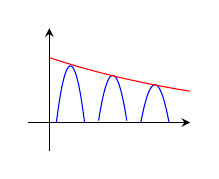
\begin{tikzpicture}
   \begin{axis}[
       width=0.3\textwidth,
       axis lines=middle,
       no markers,
       xtick=\empty,
       ytick=\empty,
       clip=false,
       xlabel={},
       ylabel={},
       domain=-2:2,
       ymin=-0.3, ymax=1,
       xmin= -0.3, xmax=2,
       samples=100,
       view = {0}{90}
   ]
       \addplot[blue, domain=0.1:0.5] {-15*(x-0.3)^2 + 0.6};
       \addplot[blue, domain=0.7:1.1] {-12*(x-0.9)^2 + 0.5};
       \addplot[blue, domain=1.3:1.7] {-10*(x-1.5)^2 + 0.4};
       \addplot[red, domain=0:2] {0.688883*0.69359^x};


   \end{axis}
   \end{tikzpicture}
   \end{center}

   Though we still want to recover the envelope (all the information is in the amplitude of the envelope).

   \begin{center}
    \begin{circuitikz}[american voltages]
         \node at (-0.5, 0) {$r(t)$}; 
         \draw (0, 0) to[diode] (2, 0)
             to[resistor] (2, -2)
             -- (2, -2) node[below, ground] {} ;
 
         \draw (2, 0) -- ++(2, 0) to[capacitor] ++(0, -2) -- ++(-2, 0);
         \draw (4, 0) -- ++(1, 0) node[right] {$\hat m(t)$};
 
    \end{circuitikz}
   \end{center}

\tbf{Motivating FM:}
\[r(t) = \sin\left(2\pi f_c t + \int_{-\infty}^t m(\tau) d\tau \right) \]

Where is the information here? In the integral. 

What does it look like? First, we know it has constant amplitude (``modulus 1'').

Define the \emph{instantaneous frequency} 
\[\omega(t) = \frac{d}{dt} \Theta(t) = 2\pi f_0 = \omega_0\]
for $\Theta(t) = 2\pi f_0 t$ the \emph{instantaneous phase} of the signal.

Now let's try differentiating:

\begin{align*}
    \frac{d}{dt} r(t) &= (2\pi f_c + m(t)) \cos \left(2\pi f_c t + \int_{-\infty}^t m(\tau)\; d\tau\right) 
\end{align*}

\end{document}

